\documentclass[25pt, a0paper, portrait, margin=10mm, innermargin=15mm,
blockverticalspace=15mm, colspace=15mm, subcolspace=8mm]{tikzposter}
\usepackage{natbib}
%\usepackage{pgfplots}
\usepackage[default]{lato}
\usepackage{concrete}
\usepackage[utf8]{inputenc}
\usepackage{graphics}
%\pgfplotsset{/pgf/number format/use comma,compat=1.7}

\definecolor{blau1}{RGB}{0,105,170}
\definecolor{blau2}{RGB}{80,170,200}
\definecolor{rot}{RGB}{198,24,38}
\definecolor{sand}{RGB}{244,241,234}
\definecolor{braun}{RGB}{89,13,8}
\definecolor{green}{RGB}{77,175,74}
\definecolor{red}{RGB}{228,26,28}
\definecolor{purple}{RGB}{152,78,163}
\definecolor{blue}{RGB}{55,126,184}
\tikzstyle{nonterm}=[rounded corners,draw=blue!50,fill=blue!20,thick,font=\sffamily]
\tikzstyle{vroot}=[rounded corners,draw=gray!50,fill=gray!20,thick,font=\sffamily]
\tikzstyle{nontermedge}=[line width=1.5pt,draw=black!50]
\tikzstyle{vrootedge}=[line width=1.5pt,draw=gray!20]
\tikzstyle{termcell}=[matrix,inner sep=1pt,row sep=0pt,matrix anchor=north west]
\tikzstyle{terminal}=[rectangle,font=\small]
\tikzstyle{edgelabel}=[rectangle,draw=gray!50,fill=gray!20,font=\sffamily\tiny]

\usecolorstyle[colorTwo=braun,colorThree=sand,colorOne=rot]{Australia}
\colorlet{notebgcolor}{rot}

\titlegraphic{
\includegraphics[height=8cm]{logo-University-of-Heidelberg.jpg}}
\title{Rule-based Corefence Resolution with BART}
\institute{Institute for Computational Linguistics, Univ. Heidelberg}
\author{Julian Baumann, Xenia Kühling, Sebastian Ruder}
\makeatletter
\makeatother

\begin{document}\maketitle

%\begin{columns} \column{1.0}
%\block{Goal}
%	{	
%Improvement of coreference resolution through integration of the rule-based, entity-centric Stanford sieve architecture into the existing BART machine learning system.  
%
%	} 
%	\end{columns}

\begin{columns} 
	

\column{0.6} 
\block{Goal}
	{	
Improvement of coreference resolution through integration of the rule-based, entity-centric Stanford sieve architecture into the existing BART machine learning system.  

	} 
\block{Stanford Coreference System}{
\begin{tikzfigure}[Functionality of Stanford Coreference System]
%\begin{tikzpicture}
%stanford.png
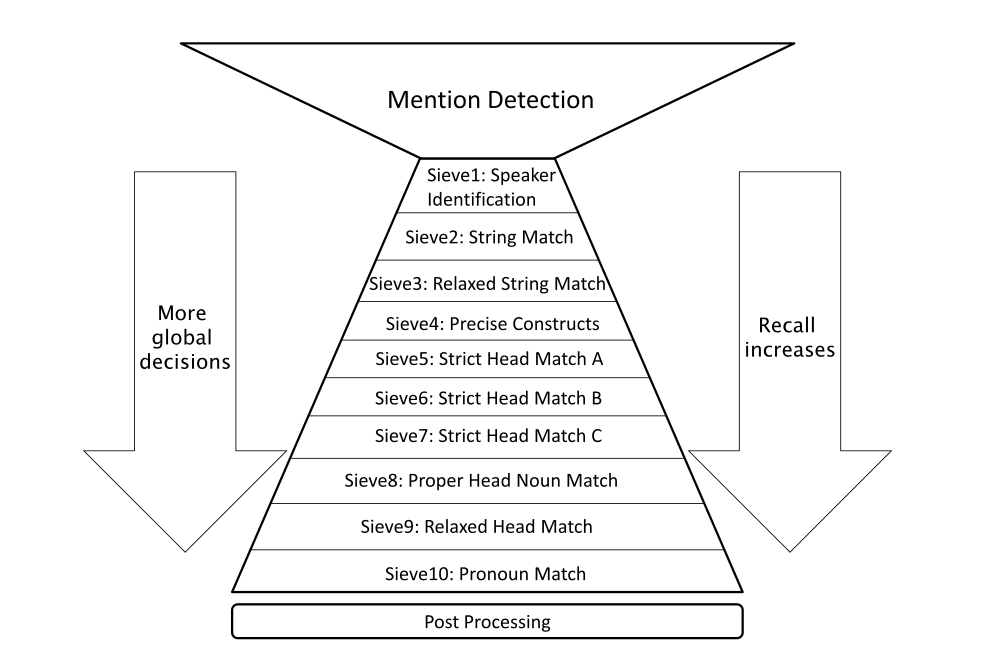
\includegraphics[scale=0.7]{stanford.png}
%\end{tikzpicture}
\end{tikzfigure}
\begin{itemize}
\item Input (mentions) passes ten independent precision-oriented coreference models ("sieves")
\item Entity-centric approach uses previous sieves' output and information to make decisions
\end{itemize}}

\block{Examples}{
%\textbf{[Der koreanische Autokonzern Daewoo]}$^{1}_{1}$ wollte auf [keinen Fall]$^{2}_{2}$ mit [\textbf{[seinem]}$^{1}_{3}$ Autoumschlag]$^{3}_{4}$ in [Bremerhaven]$^{4}_{5}$ bleiben und mit [\textbf{[seiner]}$^{1}_{6}$ Konzern-Zentrale]$^{5}_{7}$ auch nicht nach [Bremerhaven]$^{4}_{8}$ gehen.   
% 
%\begin{quote}\texttt{Antecedent of '[seinem]':'[Der koreanische Autokonzern Daewoo]' with PronounMatchSieve\\
%Antecedent of '[seiner]':'[Der koreanische Autokonzern Daewoo]' with PronounMatchSieve
%}\\
%\end{quote}
%
%Dafür spricht \textbf{[[ihre]$^{1}_{1}$ klassische Ausbildung]}$^{2}_{2}$,  \textbf{[die]}$^{2}_{3}$ nicht mit [Wegwerfkultur]$^{3}_{4}$ und platten Melodien zusammen paßt.
%\begin{quote}\texttt{Antecedent of '[die]':'[ihre klassische Ausbildung]' with PreciseConstructSieve
%}\\
%\end{quote}
%
%"\textbf{[Ich]}$^{1}_{1}$ schließe jetzt ab", sagt \textbf{[der Standesbeamte Rolf Paschen]}$^{1}_{2}$ resolut, "sonst wird das hier nie was."
%
%\begin{quote}\texttt{Antecedent of '[der Standesbeamte Rolf Paschen]':'[Ich]' with SpeakerIdentificationSieve
%}\\
%\end{quote}

\innerblock{Precise Constructs Sieve}
{Dafür spricht \textbf{[[ihre]$^{1}_{1}$ klassische  Ausbildung]}$^{2}_{2}$,  \textbf{[die]}$^{2}_{3}$ nicht mit [Wegwerfkultur]$^{3}_{4}$ und platten Melodien zusammen paßt.
\begin{quote}
\texttt{TRUE! Antecedent of '[die]':'[ihre klassische Ausbildung]'}
\end{quote}}

\innerblock{Pronoun Match Sieve}
{\textbf{[Der koreanische Autokonzern Daewoo]}$^{1}_{1}$ wollte auf [keinen Fall]$^{2}_{2}$ mit [\textbf{[seinem]}$^{1}_{3}$ Autoumschlag]$^{3}_{4}$ in [Bremerhaven]$^{4}_{5}$ bleiben und mit [\textbf{[seiner]}$^{1}_{6}$ Konzern-Zentrale]$^{5}_{7}$ auch nicht nach [Bremerhaven]$^{4}_{8}$ gehen.
\begin{quote}
\texttt{TRUE! Antecedent of '[seinem]':'[Der koreanische Autokonzern Daewoo]' \\
TRUE! Antecedent of '[seiner]':'[Der koreanische Autokonzern Daewoo]'}
\end{quote}}

\innerblock[]{Speaker Identification Sieve}{"\textbf{[Ich]}$^{1}_{1}$ schließe jetzt ab", sagt \textbf{[der Standesbeamte Rolf Paschen]}$^{1}_{2}$ resolut, "sonst wird das hier nie was."
\begin{quote}
\texttt{TRUE! Antecedent of '[der Standesbeamte Rolf Paschen]':'[Ich]'}
\end{quote}}


\innerblock
{Entities that require more or commonsense knowledge}
{\textbf{[Der Saatgutkonzern Pioneer Hi-Bred]}$^{1}_{1}$ hat in [Süddeutschland]$^{2}_{2}$ [nicht zugelassenen Gentech-Mais]$^{3}_{3}$ verkauft.\\\textbf{[Der Weltmarktführer für [Saatgut]$^{4}_{4}$]}$^{1}_{5}$ verstößt damit gegen [das Gentechnikgesetz]$^{5}_{6}$, [...].
\begin{quote}
\texttt{FALSE! No Antecedent for '[Der Weltmarktführer für Saatgut]'\\ANTECEDENT: [Der Saatgutkonzern Pioneer]}
\end{quote}}
} 
%\note[targetoffsetx = 9cm, targetoffsety = -15.5 cm]{Rule-based approach not working!}


%
%\block{Problems}{
%\innerblock
%{Entities that require more or commonsense knowledge}
%{\textbf{[Der Saatgutkonzern Pioneer Hi-Bred]}$^{1}_{1}$ hat in [Süddeutschland]$^{2}_{2}$ [nicht zugelassenen Gentech-Mais]$^{3}_{3}$ verkauft.\\\textbf{[Der Weltmarktführer für [Saatgut]$^{4}_{4}$]}$^{1}_{5}$ verstößt damit gegen [das Gentechnikgesetz]$^{5}_{6}$, [...].
%\begin{quote}
%\texttt{FALSE! No Antecedent for '[Der Weltmarktführer für Saatgut]'\\ANTECEDENT: [Der Saatgutkonzern Pioneer]}
%\end{quote}}
%} 


\column{0.4}


\block{BART}{
\begin{tikzfigure}[Functionality of BART]
%\begin{tikzpicture}
%stanford.png
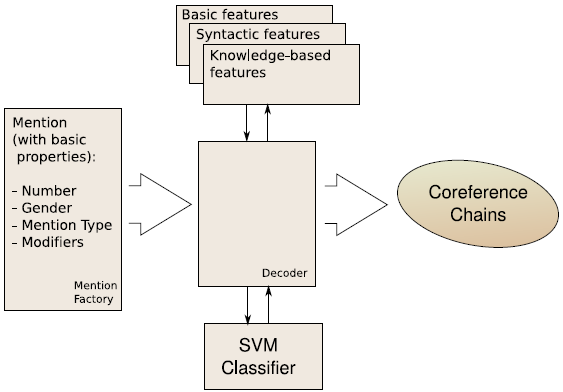
\includegraphics{bart_summary.png}
%\end{tikzpicture}
\end{tikzfigure}
\begin{itemize}
\item Mentions containing semantic information about a markable (gender, number, etc.) are generated
\item Machine Learning employs syntactic and semantic features to generate pair instances (anaphor, antecedent) which are assembled in coreference chains
\end{itemize}}



\block{Evaluation}
	{
For German we used the first 100 documents of TüBa-D/Z (2008) to evaluate our system.
To compare it to the original English based Stanford Sieve System, we also evaluated  it
on CoNLL-2011 Shared Task training set. 
\begin{tikzfigure}[\textit{GERMAN}: Comparison with BART ML Configuration (\texttt{XMLExperiment} ) ]	
\begin{tabular}{l||ll|l}
& \multicolumn{3}{c}{\textbf{MUC-Score}} \\ \hline
               & \textbf{Recall}		 & \textbf{Precision} & \textbf{F\_1}    \\ \hline
Our System 	& 0.644      & 0.691              & 0.667  \\
BART  & 0.721 		 & 0.532     & 0.612
\end{tabular}
\end{tikzfigure}


\begin{tikzfigure}[\textit{GERMAN}: Performance of individual sieves  ]
\begin{tabular}{l||ll|l}
& \multicolumn{3}{c}{\textbf{MUC-Score}} \\ \hline
	                 & \textbf{Recall} & \textbf{Precision} & \textbf{F\_1} \\ \hline
SpeakerIdentification & 0.004 & 0.637 & 0.008 \\
+StringMatch & 0.157 & 0.857 & 0.265 \\
+RelaxedStringMatch & 0.180 & 0.825 & 0.295 \\
+PreciseConstructs & 0.241 & 0.822 & 0.372 \\
+HeadMatchA & 0.295 & 0.809 & 0.432 \\
+HeadMatchB & 0.355 & 0.775 & 0.487 \\
+HeadMatchC & 0.357 & 0.771 & 0.488 \\
+ProperHeadNounMatch & 0.358 & 0.771 & 0.489 \\
+RelaxedHeadMatch & 0.383 & 0.771 & 0.512 \\
+PronounMatch & 0.644 & 0.691 & 0.667 \\ 
\end{tabular}
\end{tikzfigure}

\begin{tikzfigure}[\textit{ENGLISH}: Comparison with Stanford System ]
\begin{tabular}{l|ll|l}
& \multicolumn{1}{c}{\textbf{MUC-Score}} \\ \hline
          &    \textbf{F\_1}    \\ \hline
Our System &	  0.420  \\
Stanford   &	0.603
\end{tabular}
\end{tikzfigure}
	}

	
\end{columns}
	
	\begin{columns} \column{1.0}
\block{Conclusion}
	{
The rule-based sieve approach exceeds ML performance. Because our system has been designed primarily using linguistic constants specific to German, there still remains a lot of room for improvement for the English language. Due to the nature of the rule-based approach, the system is easy to extend. We leave this along with its adaptation to English, Italian, and other languages as future work.
	}
	


\end{columns}

\column{1}
\block{References}{
\small{
Broscheit, S. et al. (2010), BART: A multilingual anaphora resolution system, in ‘Pro-
ceedings of the 5th International Workshop on Semantic Evaluation’, SemEval ’10,
Association for Computational Linguistics, Stroudsburg, PA, USA, pp. 104–107.\\
Lee, H. et al. (2013), ‘Deterministic coreference resolution based on entity-centric,
precision-ranked rules’, Comput. Linguist. 39(4), 885–916.\\
Versley, Y. et al. (2008), BART: A modular toolkit for coreference resolution, in ‘Pro-
ceedings of the ACL-08: HLT Demo Session’, Association for Computational Lin-
guistics, Columbus, Ohio, pp. 9–12.\\
}}

\end{document}
